We describe how to use causality for a given DyNetKAT expression.

\begin{definition}
    Given sets of events $E_0$ and $E_1$ let
    $E = \s{(0,e)|e \in E_0} \cup \s{(1,e)|e \in E_1}$.
    We define injections $\iota_k: E_k \rightarrow E$, given by
    $\iota_k(e) = (k,e)$, for $k = 0,1$.
\end{definition}

\begin{definition}
    Given sets of events $E_0$ and $E_1$ let their product $E$ be:
    \begin{align*}
        E_0 \times_* E_1 = \s{(e_0,*)|e_0 \in E_0} \cup \s{(*,e_1)|e_1 \in E_1}
        \cup \s{(e_0,e_1)|e_0 \in E_0 \wedge e_1 \in E_1}
    \end{align*}
    We define projections $\pi_i: E \rightarrow_* E_i$, given by
    $\pi_i(e_0,e_1) = e_i$, for $i=0,1$.
\end{definition}

\begin{definition}
    Let $\mathrm{E} = (E,\#,\vdash,L,l)$ be a labeled event structure and
    $M$ be its causal model with the set of variables:
    \begin{align*}
        \mathcal{V} = & \s{C_{e_i,e_j} |  1 \leq i < j \leq n.
        e_i \in E \amp e_j \in E}                                \\
                      & \cup \s{EN_{s,e} | s \in \mathcal{P}(E),
            e \in E. e \not \in s }
    \end{align*}
    Let $\alpha$ be a label and $\mathrm{E'} = \alpha \mathrm{E}$.
    We define $M' = \alpha M$ to be a causal model where:
    \begin{align*}
        \mathcal{V'} = & \s{C'_{e_i,e_j} |  1 \leq i < j \leq n.
        e_i \in E' \amp e_j \in E'}                                 \\
                       & \cup \s{EN'_{s,e} | s \in \mathcal{P}(E'),
        e \in E'. e \not \in s }                                    \\
                       & \cup \mathcal{V}
    \end{align*}
    Next, we define functions of $M'$ as follows:
    $$
        \f{C'_{e,e'}} = \begin{cases}
            \T       & \text{ if } e = \iota_0(\alpha) \vee e' = \iota_0(\alpha) \\
            C_{e,e'} & \text{ otherwise }
        \end{cases}
    $$

    $$
        \f{EN'_{s,e}} = \begin{cases}
            Con(s)                  & \text{ if } e = \iota_0(\alpha)             \\
            EN_{s',e} \wedge Con(s) & \text{ if } s = s' \cup \s{\iota_0(\alpha)} \\
            \F                      & \text{ otherwise }
        \end{cases}
    $$
\end{definition}

\begin{definition}
    Let $\mathrm{E}_0 = (E_0,\#_0,\vdash_0,L_0,l_0)$ and
    $\mathrm{E}_1 = (E_1,\#_1,\vdash_1,L_1,l_1)$ be labeled event structures
    and $M_0,M_1$ be their causal models.
    Let $(E',\#',\vdash',L',l') = \mathrm{E_0} + \mathrm{E_1}$.
    We define $M' = M_0 + M_1$ to be a causal model where we have:
    \begin{align*}
        \mathcal{V}_0 = & \s{C_{e_i,e_j}^0 |  1 \leq i < j \leq n.
        e_i \in E_0 \amp e_j \in E_0}                                 \\
                        & \cup \s{EN_{s,e}^0 | s \in \mathcal{P}(E_0)
        e \in E_0. e \not \in s }                                     \\
        \mathcal{V}_1 = & \s{C_{e_i,e_j}^1 |  1 \leq i < j \leq n.
        e_i \in E_1 \amp e_j \in E_1}                                 \\
                        & \cup \s{EN_{s,e}^1 | s \in \mathcal{P}(E_1)
        e \in E_1. e \not \in s }                                     \\
        \mathcal{V} =   & \s{C_{e_i,e_j} |  1 \leq i < j \leq n.
        e_i \in E' \amp e_j \in E'}                                   \\
                        & \cup \s{EN_{s,e} | s \in \mathcal{P}(E'),
        e \in E'. e \not \in s }                                      \\
                        & \cup \mathcal{V}_0 \cup \mathcal{V}_1
    \end{align*}
    We define the functions of $M'$ as follows:
    $$
        \f{C_{e,e'}} = \begin{cases}
            \T         & \text{ if } \exists e_0 \in E_0,e_1 \in E_1.
            (e = \iota_0(e_0) \wedge e' = \iota_1(e_1))
            \vee (e' = \iota_0(e_0) \wedge e = \iota_1(e_1))                    \\
            C^0_{e,e'} & \text{ if } \exists e_0,e_0' \in E_0. e = \iota_0(e_0)
            \wedge e' = \iota_0(e_0')                                           \\
            C^1_{e,e'} & \text{ if } \exists e_1,e_1' \in E_1. e = \iota_1(e_1)
            \wedge e' = \iota_1(e_1')
        \end{cases}
    $$
    $$
        \f{EN_{s,e}} = \begin{cases}
            Con(s) \wedge EN^0_{s_0,e_0} & \text{ if }
            \exists s_0 \in Con_0,e_0 \in E_0. s = \iota_0(s_0)
            \wedge e = \iota_0(e_0)                           \\
            Con(s) \wedge EN^1_{s_1,e_1} & \text{ if }
            \exists s_1 \in Con_1,e_1 \in E_1. s = \iota_1(s_1)
            \wedge e = \iota_1(e_1)                           \\
            \F                           & \text{ otherwise }
        \end{cases}
    $$
\end{definition}

\begin{definition}
    Let $\mathrm{E}_0 = (E_0,\#_0,\vdash_0,L_0,l_0)$ and
    $\mathrm{E}_1 = (E_1,\#_1,\vdash_1,L_1,l_1)$ be event structures and
    $M_0,M_1$ be their causal models.
    Let $(E',\#',\vdash',L',l') = E_0 \times E_1$.
    We define $M' = M_0 \times M_1$ to be a causal model where we have:
    \begin{align*}
        \mathcal{V}_0 = & \s{C_{e_i,e_j}^0 |  1 \leq i < j \leq n.
        e_i \in E_0 \amp e_j \in E_0}                                 \\
                        & \cup \s{EN_{s,e}^0 | s \in \mathcal{P}(E_0)
        e \in E_0. e \not \in s }                                     \\
        \mathcal{V}_1 = & \s{C_{e_i,e_j}^1 |  1 \leq i < j \leq n.
        e_i \in E_1 \amp e_j \in E_1}                                 \\
                        & \cup \s{EN_{s,e}^1 | s \in \mathcal{P}(E_1)
        e \in E_1. e \not \in s }                                     \\
        \mathcal{V} =   & \s{C_{e_i,e_j} |  1 \leq i < j \leq n.
        e_i \in E' \amp e_j \in E'}                                   \\
                        & \cup \s{EN_{s,e} | s \in \mathcal{P}(E'),
        e \in E'. e \not \in s }                                      \\
                        & \cup \mathcal{V}_0 \cup \mathcal{V}_1
    \end{align*}
    We define the functions of $M'$ as follows:
    $$
        \f{C_{e,e'}} = \begin{cases}
            \T & \text{ if } \pi_0(e) = \pi_0(e') \vee \pi_1(e) = \pi_1(e') \\
            C^0(\pi_0(e),\pi_0(e')) \vee  C^1(\pi_1(e),\pi_1(e'))
               & \text { if } \pi_0(e) \neq * \wedge \pi_1(e) \neq *        \\
            C^0(\pi_0(e),\pi_0(e'))
               & \text { if } \pi_1(e) = *                                  \\
            C^1(\pi_1(e),\pi_1(e'))
               & \text { if } \pi_0(e) = *                                  \\
        \end{cases}
    $$
    $$
        \f{EN_{s,e}} = \begin{cases}
            EN^0(\pi_0(s),\pi_0(e)) \wedge EN^1(\pi_1(s),\pi_1(e))
                                    & \text{ if } \pi_0(e) \neq * \wedge \pi_1(e) \neq * \\
            EN^0(\pi_0(s),\pi_0(e)) & \text{ if } \pi_1(e) = *                           \\
            EN^1(\pi_1(s),\pi_1(e)) & \text{ if } \pi_0(e) = *                           \\
        \end{cases}
    $$
\end{definition}
\begin{definition}
    Let $\mathrm{E} = (E,\#,\vdash,L,l)$ be an event structure and $M$ its
    causal model.
    For each variable $v \in \mathcal{V}$ we define a function $l(v)$ which
    returns the set of labels of this variable regarding the $l$ as follows:
    $$
        l(v) = \begin{cases}
            \s{l(e),l(e')}                     & \text{ if } \exists e,e' \in E. v = C_{e,e'} \\
            \s{l(e')| e' \in s } \cup \s{l(e)} & \text{ if }
            \exists s \subseteq E, e \in E. v = EN_{s,e}
        \end{cases}
    $$
\end{definition}

\begin{definition}
    Let $\mathrm{E} = (E,\#,\vdash,L,l)$ be an event structure and $M$ its
    causal model.
    Given a set of labels $\Lambda$, we define $M' = M\lceil \Lambda$ to be
    a causal model where we have removed any variable such as
    $x \in \mathcal{V}$ and its functions where $l(v) \not \subseteq \Lambda$.
\end{definition}

\begin{example}
    Consider the following network where we want to check a blacklist
    property, i.e. no packets arrive at $c$:
    \begin{center}
        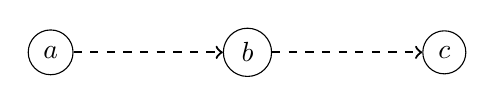
\begin{tikzpicture}[node distance={25mm},
                main/.style = {draw, circle},
                d/.style = {->,thick,dashed} ]
            \node[main] (a) {$a$};
            \node[main] (b) [right of=a] {$b$};
            \node[main] (c) [right of=b] {$c$};
            \draw[d] (a) -- (b);
            \draw[d] (b) -- (c);
        \end{tikzpicture}
    \end{center}
    We define this network using the following DyNetKAT term:
    \begin{align*}
        S_{xy}  & = sw = x \cdot sw \la y            \\
        P       & = u!S_{ab}                         \\
        Q       & = u!S_{bc}                         \\
        N_{x,y} & = (S_x+S_y)^* \oplus u?x';N_{x',y}
        \oplus u?y';N_{x,y'}                         \\
        SDN     & = N_{0,0} \parallel P \parallel Q
    \end{align*}
    We may rewrite the terms as follows:
    \begin{align*}
        N_{0,0}   & = u?S_{ab};N_{ab,0} \oplus u?S_{bc};N_{0,bc} \\
        N_{ab,0}  & = S_{ab}^* \oplus u?S_{bc};N_{ab,bc}         \\
        N_{0,bc}  & = S_{bc}^* \oplus u?S_{ab};N_{ab,cd}         \\
        N_{ab,bc} & = (S_{ab}+S_{bc})^*
    \end{align*}
    We consider this network under the situation that a single packet
    arrived at $a$.
    Thus we assume that a single packet $\sigma$ is arrived where
    $\sigma(sw) = a$.
    Under this condition, we can replace the NetKAT terms with
    packet forwarding actions of the form $(\sigma, \sigma')$.
    We use $xy$ to denote an action of the form $(\sigma,\sigma')$
    where $\sigma(sw) = x$ and $\sigma'(sw) = y$.
    For a DyNetKAT term $T$, we use $T^a$ to denote the term where
    we have replaced all NetKAT policies with packet forwarding actions.
    Given a packet $\sigma$ where $\sigma(l) = a$ we can replace NetKAT
    Furthermore, we rename actions
    $u?S_{ab},u!S_{ab},u?S_{bc},u!S_{bc}$ to $u_a,u_a',u_b,u_b'$,
    so we can derive the following terms:
    Thus we have:
    \begin{align*}
        SDN^a       & = \delta_{\mathcal{L}}(N^a_{0,0}
        \parallel P \parallel Q)                         \\
        P^a         & = u_a'                               \\
        Q^a         & = u_b'                               \\
        N^a_{0,0}   & = u_a;N^a_{ab,0} \oplus u_b;N^a_{0,bc} \\
        N^a_{ab,0}  & = ab \oplus u_b;N^a_{ab,bc}          \\
        N^a_{0,bc}  & = u_a;N^a_{ab,bc}                    \\
        N^a_{ab,bc} & = ab \oplus ac
    \end{align*}
    Let we denote $rcfg(u_a,u_a')$ and $rcfg(u_b,u_b')$ with $p$ and $q$ 
    respectively.
    Thus we can derive the following LTS for $SDN^a$:
    \begin{center}
        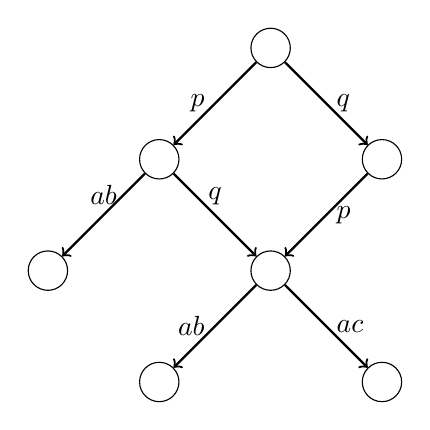
\begin{tikzpicture}[node distance={20mm},
                main/.style = {draw, circle,minimum width=5mm},
                s/.style = {->,thick}]
            \node[main] (s1) {};
            \node[main] (s2) [below left of=s1] {};
            \node[main] (s3) [below right of=s1] {};
            \node[main] (s4) [below left of=s2] {};
            \node[main] (s5) [below right of=s2] {};
            \node[main] (s6) [below left of=s5] {};
            \node[main] (s7) [below right of=s5] {};
            \draw[s] (s1) -- node[left]{$p$} (s2);
            \draw[s] (s1) -- node[right]{$q$}(s3);
            \draw[s] (s2) -- node[above]{$ab$}(s4);
            \draw[s] (s2) -- node[above]{$q$}(s5);
            \draw[s] (s3) -- node[right]{$p$}(s5);
            \draw[s] (s5) -- node[left]{$ab$}(s6);
            \draw[s] (s5) -- node[right]{$ac$}(s7);
        \end{tikzpicture}
    \end{center}
    Let $\mathrm{E} = (E,\#,\vdash,L,l)$ be the event structure of $SDN^a$
    where $L = \s{p,q,ab,ac}$.
    We define the blacklist property as follows:
    \begin{align*}
        P = \s{s \in \mathcal{P}| \forall e \in s. l(e) \neq ac}
    \end{align*}  
\end{example}